% Options for packages loaded elsewhere
\PassOptionsToPackage{unicode}{hyperref}
\PassOptionsToPackage{hyphens}{url}
%
\documentclass[
  12pt,
]{article}
\usepackage{amsmath,amssymb}
\usepackage{lmodern}
\usepackage{iftex}
\ifPDFTeX
  \usepackage[T1]{fontenc}
  \usepackage[utf8]{inputenc}
  \usepackage{textcomp} % provide euro and other symbols
\else % if luatex or xetex
  \usepackage{unicode-math}
  \defaultfontfeatures{Scale=MatchLowercase}
  \defaultfontfeatures[\rmfamily]{Ligatures=TeX,Scale=1}
\fi
% Use upquote if available, for straight quotes in verbatim environments
\IfFileExists{upquote.sty}{\usepackage{upquote}}{}
\IfFileExists{microtype.sty}{% use microtype if available
  \usepackage[]{microtype}
  \UseMicrotypeSet[protrusion]{basicmath} % disable protrusion for tt fonts
}{}
\makeatletter
\@ifundefined{KOMAClassName}{% if non-KOMA class
  \IfFileExists{parskip.sty}{%
    \usepackage{parskip}
  }{% else
    \setlength{\parindent}{0pt}
    \setlength{\parskip}{6pt plus 2pt minus 1pt}}
}{% if KOMA class
  \KOMAoptions{parskip=half}}
\makeatother
\usepackage{xcolor}
\IfFileExists{xurl.sty}{\usepackage{xurl}}{} % add URL line breaks if available
\IfFileExists{bookmark.sty}{\usepackage{bookmark}}{\usepackage{hyperref}}
\hypersetup{
  pdftitle={Exercise 3: The Phillips Curve},
  pdfauthor={Stefano Graziosi},
  hidelinks,
  pdfcreator={LaTeX via pandoc}}
\urlstyle{same} % disable monospaced font for URLs
\usepackage[margin=1in]{geometry}
\usepackage{graphicx}
\makeatletter
\def\maxwidth{\ifdim\Gin@nat@width>\linewidth\linewidth\else\Gin@nat@width\fi}
\def\maxheight{\ifdim\Gin@nat@height>\textheight\textheight\else\Gin@nat@height\fi}
\makeatother
% Scale images if necessary, so that they will not overflow the page
% margins by default, and it is still possible to overwrite the defaults
% using explicit options in \includegraphics[width, height, ...]{}
\setkeys{Gin}{width=\maxwidth,height=\maxheight,keepaspectratio}
% Set default figure placement to htbp
\makeatletter
\def\fps@figure{htbp}
\makeatother
\setlength{\emergencystretch}{3em} % prevent overfull lines
\providecommand{\tightlist}{%
  \setlength{\itemsep}{0pt}\setlength{\parskip}{0pt}}
\setcounter{secnumdepth}{-\maxdimen} % remove section numbering
\usepackage{amsmath}
\usepackage{amssymb}
\usepackage{float}
\usepackage{booktabs}
\usepackage{float}
\usepackage{longtable}
\usepackage{array}
\usepackage{multirow}
\usepackage{wrapfig}
\usepackage{colortbl}
\usepackage{pdflscape}
\usepackage{tabu}
\usepackage{threeparttable}
\usepackage{threeparttablex}
\usepackage[normalem]{ulem}
\usepackage{makecell}
\usepackage{xcolor}
\ifLuaTeX
  \usepackage{selnolig}  % disable illegal ligatures
\fi

\title{Exercise 3: The Phillips Curve}
\usepackage{etoolbox}
\makeatletter
\providecommand{\subtitle}[1]{% add subtitle to \maketitle
  \apptocmd{\@title}{\par {\large #1 \par}}{}{}
}
\makeatother
\subtitle{Problem Set 4 --- Macroeconomics (20285)}
\author{Stefano Graziosi}
\date{April 27, 2026}

\begin{document}
\maketitle

\newpage

\hypertarget{section-3.1-the-classic-phillips-curve}{%
\section{Section 3.1 --- The Classic Phillips
Curve}\label{section-3.1-the-classic-phillips-curve}}

\hypertarget{question-1-backward-looking-inflation-expectations}{%
\subsection{Question 1: Backward-Looking Inflation
Expectations}\label{question-1-backward-looking-inflation-expectations}}

\textbf{Answer:} The backward-looking measure
\(\tilde{E}_t[\pi_{t+1}] = \frac{1}{4}(\pi_{t-1} + \pi_{t-2} + \pi_{t-3} + \pi_{t-4})\)
embodies an \emph{adaptive expectations} hypothesis: agents form their
forecast of next-period inflation by simply averaging the four most
recent quarterly inflation outcomes. Because it is a four-quarter moving
average, this series is mechanically smoother than actual inflation ---
it dampens transitory spikes and responds only gradually to persistent
shifts. The measure implicitly assumes that agents use \emph{only} past
own-inflation to forecast, ignoring all other potentially informative
variables (monetary policy announcements, survey data, commodity prices,
etc.). This is a strong assumption, and it means the measure will
systematically lag behind turning points in actual inflation and may
fail to capture the forward-looking component of expectations that
drives pricing decisions.

\newpage

\hypertarget{question-2-full-sample-phillips-curve-scatterplot}{%
\subsection{Question 2: Full-Sample Phillips Curve
Scatterplot}\label{question-2-full-sample-phillips-curve-scatterplot}}

\begin{figure}[H]

{\centering 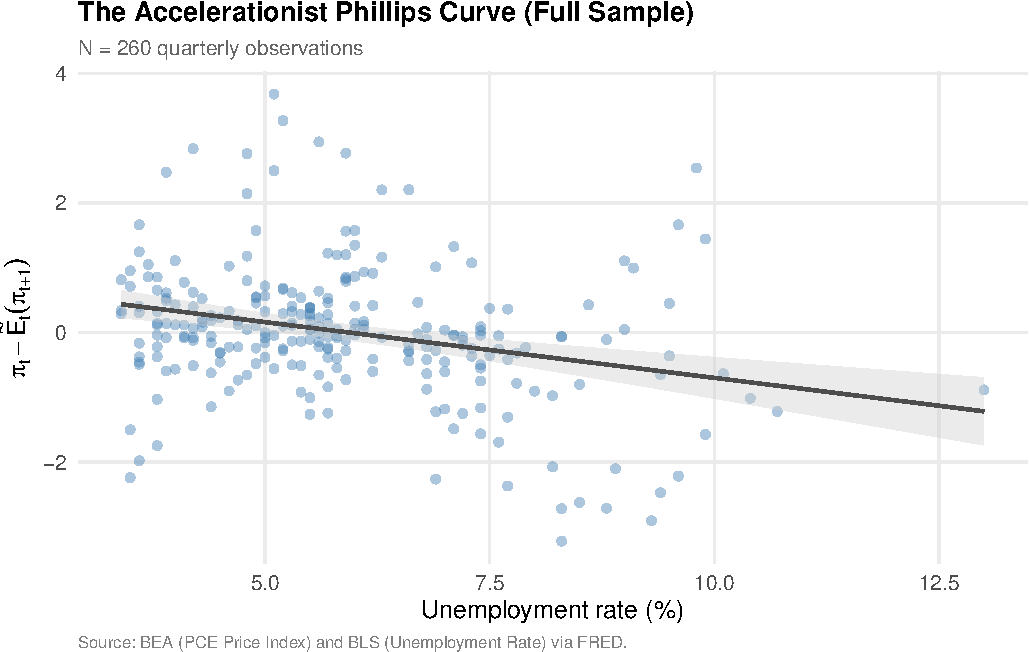
\includegraphics[width=0.9\linewidth]{../report/images/q2-scatterplot-1} 

}

\caption{Full-sample accelerationist Phillips curve: inflation surprise vs.\ unemployment rate.}\label{fig:q2-scatterplot}
\end{figure}

\textbf{Answer:} The dependent variable
\(y_t = \pi_t - \tilde{E}_t[\pi_{t+1}]\) measures the \emph{inflation
surprise} --- the deviation of realised inflation from backward-looking
expected inflation. A negative slope coefficient on \(u_t\) is
consistent with the Phillips curve: when unemployment is high, inflation
tends to come in \emph{below} expectations. The full-sample OLS fit
(\(\hat{\kappa} = -0.172\) (HC1 SE \(= 0.044\)), \(R^2 = 0.081\),
\(N = 260\)) confirms a small but statistically significant negative
slope. The economic magnitude is modest and the \(R^2\) low, reflecting
the well-known instability of the reduced-form Phillips curve: much of
the variation in inflation surprises is driven by supply shocks,
expectation shifts, and regime changes that are not captured by a simple
bivariate regression on unemployment.

\newpage

\hypertarget{question-3-subperiod-phillips-curves}{%
\subsection{Question 3: Subperiod Phillips
Curves}\label{question-3-subperiod-phillips-curves}}

\begin{figure}[H]

{\centering 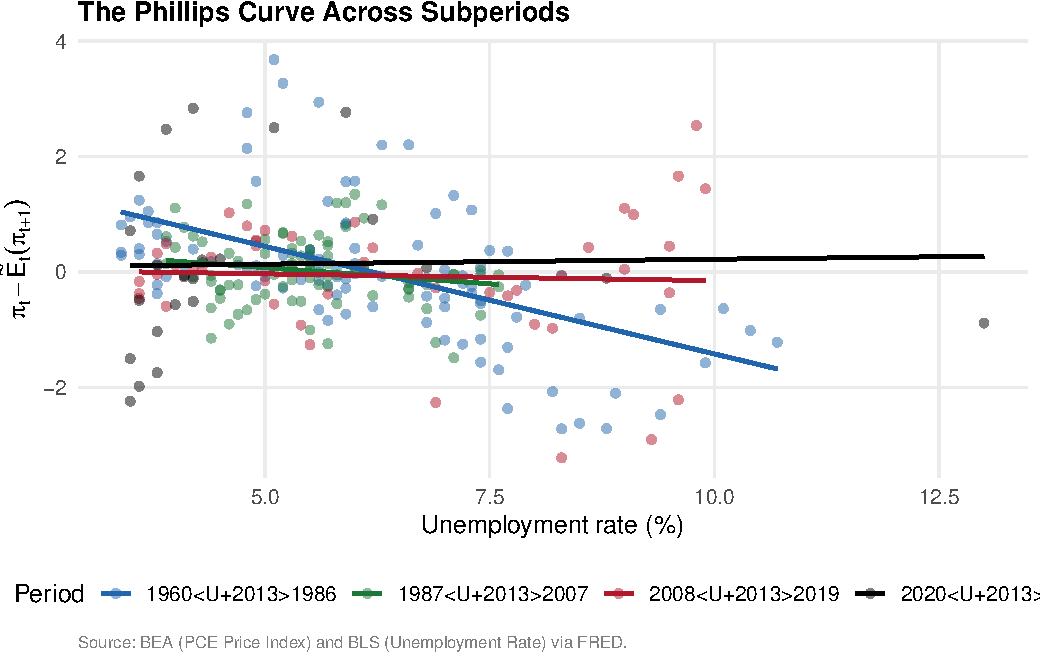
\includegraphics[width=0.9\linewidth]{../report/images/q3-subperiods-1} 

}

\caption{Phillips curve by subperiod, each with its own OLS fit.}\label{fig:q3-subperiods}
\end{figure}

\begin{table}[!h]
\centering
\caption{\label{tab:q3-coefficients}Phillips-curve slope by subperiod (HC1-robust SEs)}
\centering
\fontsize{10}{12}\selectfont
\begin{tabular}[t]{lrrrr}
\toprule
Period & Slope ($\hat{\kappa}$) & HC1 SE & $R^2$ & $N$\\
\midrule
1960<U+2013>1986 & -0.373 & 0.050 & 0.294 & 104\\
1987<U+2013>2007 & -0.112 & 0.067 & 0.031 & 84\\
2008<U+2013>2019 & -0.024 & 0.090 & 0.002 & 48\\
2020<U+2013>2025 & 0.017 & 0.116 & 0.001 & 24\\
\bottomrule
\end{tabular}
\end{table}

\textbf{Answer:} The subperiod analysis reveals a striking
\emph{flattening} of the Phillips curve over time. During 1960--1986 ---
a period encompassing both the Great Inflation and the Volcker
disinflation --- the slope is steeply negative
(\(\hat{\kappa}\approx-0.37\)), reflecting large swings in both
unemployment and inflation surprises. The Great Moderation era
(1987--2007) shows a much flatter relationship
(\(\hat{\kappa}\approx-0.11\)): well-anchored expectations meant that
unemployment fluctuations had diminished pass-through to inflation. The
post-GFC period (2008--2019) is flatter still
(\(\hat{\kappa}\approx-0.02\), \(R^2\approx0.00\)), consistent with the
``missing disinflation'' puzzle --- unemployment rose dramatically
during and after the Great Recession, yet inflation barely fell below
expectations, suggesting that expectations anchoring (possibly to the
Fed's 2\% target) rendered the traditional trade-off nearly moot. The
COVID era (2020--2025) is harder to read: although the \emph{scatter}
spans an extraordinary range --- from the 2020:Q2 unemployment spike
paired with deflationary surprises to the 2021--2022 inflation surge at
very low \(u_t\) --- the OLS slope is statistically indistinguishable
from zero (\(\hat{\kappa}\approx 0.02\), HC1 SE \(\approx 0.12\),
\(N=24\)), because supply-driven outliers dominate a short and noisy
sample. This pattern is consistent with the idea that the Phillips curve
is non-linear and appears flat when expectations are well-anchored and
shocks are moderate, but the linear-in-\(u\) specification is poorly
suited to the COVID episode, where most of the action lies on the steep
arm of the slanted-L examined in Question\textasciitilde9.

\newpage

\hypertarget{section-3.2-household-expectations-coibion-gorodnichenko-2015}{%
\section{Section 3.2 --- Household Expectations (Coibion \&
Gorodnichenko
2015)}\label{section-3.2-household-expectations-coibion-gorodnichenko-2015}}

\hypertarget{question-4-summary-of-coibion-gorodnichenko-2015}{%
\subsection{Question 4: Summary of Coibion \& Gorodnichenko
(2015)}\label{question-4-summary-of-coibion-gorodnichenko-2015}}

\textbf{Answer:} The central question addressed by Coibion \&
Gorodnichenko (2015) is the ``missing disinflation'' puzzle: why did US
inflation not fall much further (or enter deflation) during the Great
Recession of 2008--2011, despite the massive spike in unemployment and
economic slack? Traditional Phillips curve models, which relied on
backward-looking expectations or forecasts by professionals, predicted a
much sharper disinflation.

Their key finding is that the Phillips curve is actually ``alive and
well'' once you use the \emph{correct} measure of inflation
expectations. They document that household inflation expectations (as
measured by the Michigan Survey of Consumers) closely track salient
prices, particularly oil and gasoline. During the 2009--2011 period, a
surge in global oil prices pushed household inflation expectations
higher, even as the broader economy remained in a severe slump. When
these survey-based expectations are used in an expectations-augmented
Phillips curve, the implied negative inflation surprise
(\(\pi_t - E^{MSC}_t\)) matches the high unemployment rate perfectly.
This fully explains the missing disinflation without needing to assume
that the underlying slope of the Phillips curve had flattened.

\newpage

\hypertarget{question-5-comparing-the-two-expectations-series}{%
\subsection{Question 5: Comparing the Two Expectations
Series}\label{question-5-comparing-the-two-expectations-series}}

\begin{figure}[H]

{\centering 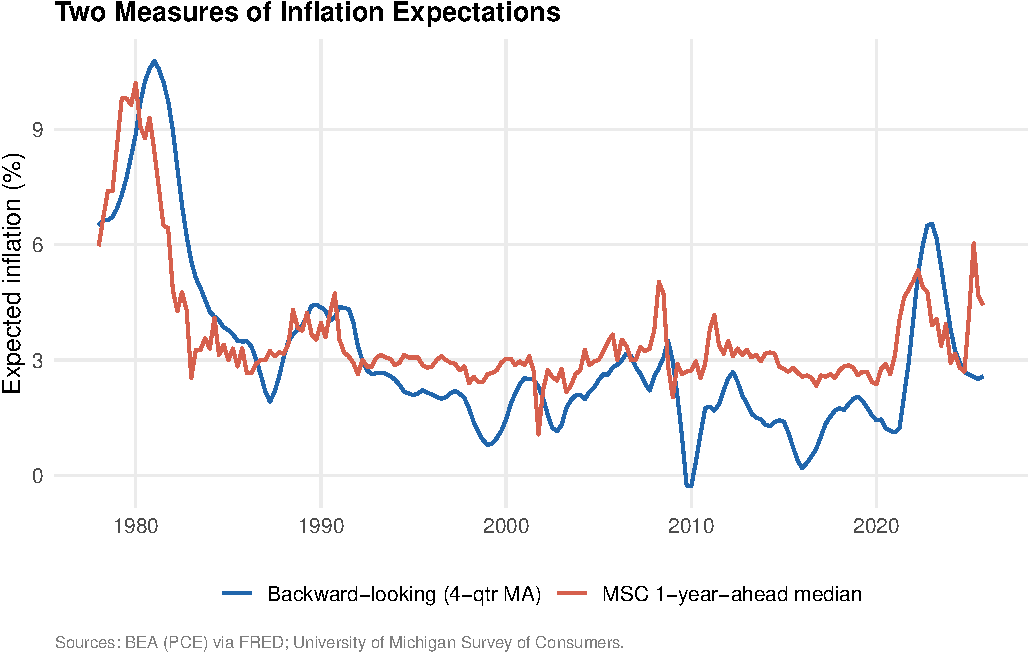
\includegraphics[width=0.9\linewidth]{../report/images/q4-comparison-1} 

}

\caption{Backward-looking vs.\ Michigan Survey household inflation expectations.}\label{fig:q4-comparison}
\end{figure}

\textbf{Answer:} Figure @ref(fig:q4-comparison) overlays the two series
on a common axis from 1978:Q1 onward. Several key differences emerge
between the backward-looking measure \(\tilde{E}_t[\pi_{t+1}]\) and the
Michigan Survey of Consumers (MSC) 1-year-ahead median expectation
\(E^{MSC}_t[\pi_{t+4}]\):

\begin{itemize}
\tightlist
\item
  \textbf{Level:} The MSC median expectation tends to run \emph{above}
  the backward-looking measure, particularly during the low-inflation
  period after 2000. Households systematically perceive and expect
  higher inflation than is recorded by the PCE index, a well-documented
  finding in the survey literature.
\item
  \textbf{Volatility:} The backward-looking measure, being a
  four-quarter moving average of actual inflation, is mechanically
  smooth. The MSC median is somewhat more volatile and can move abruptly
  in response to salient price signals (e.g., gasoline prices).
\item
  \textbf{Co-movement with actual inflation:} Both series co-move with
  actual inflation at low frequencies, but the MSC expectations diverge
  notably during the post-GFC period --- they \emph{rose} in 2009--2011
  even as actual (PCE) inflation was falling, a key insight exploited by
  Coibion \& Gorodnichenko (2015).
\end{itemize}

The \emph{median} (rather than the mean) is preferred for household
expectations because survey response distributions are typically
right-skewed and fat-tailed. A small fraction of respondents
consistently report extreme values (e.g., 20--50\% expected inflation),
which disproportionately inflate the mean. The median is robust to these
outliers and provides a more representative summary of the central
tendency of household beliefs.

\newpage

\hypertarget{question-6-phillips-curve-with-msc-expectations}{%
\subsection{Question 6: Phillips Curve with MSC
Expectations}\label{question-6-phillips-curve-with-msc-expectations}}

\begin{figure}[H]

{\centering 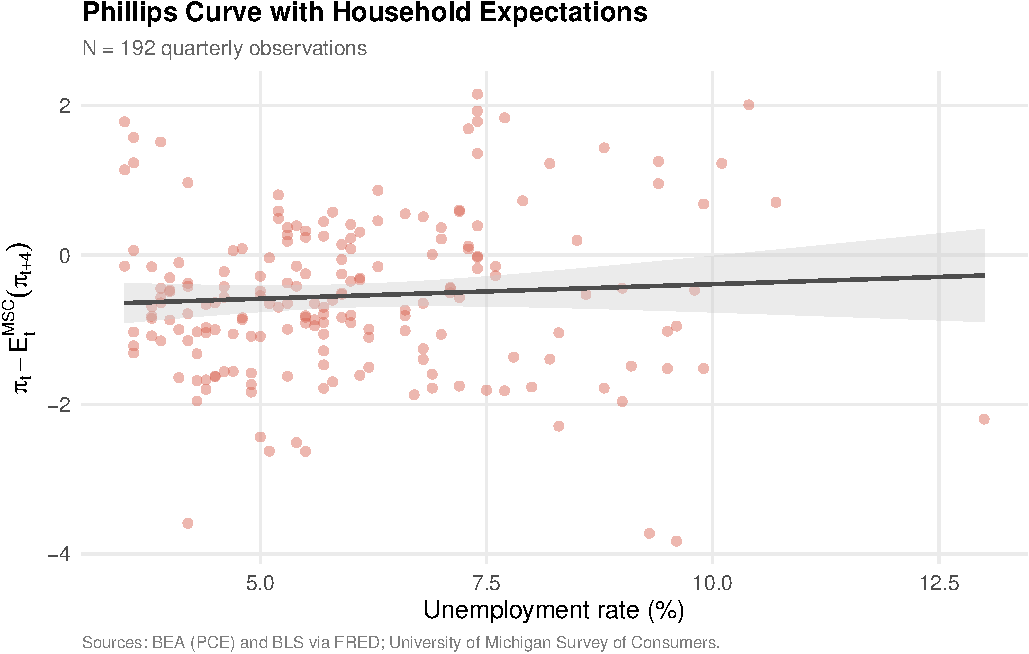
\includegraphics[width=0.9\linewidth]{../report/images/q5-msc-phillips-1} 

}

\caption{Phillips curve using MSC household expectations (contemporaneous specification).}\label{fig:q5-msc-phillips}
\end{figure}

\begin{figure}[H]

{\centering 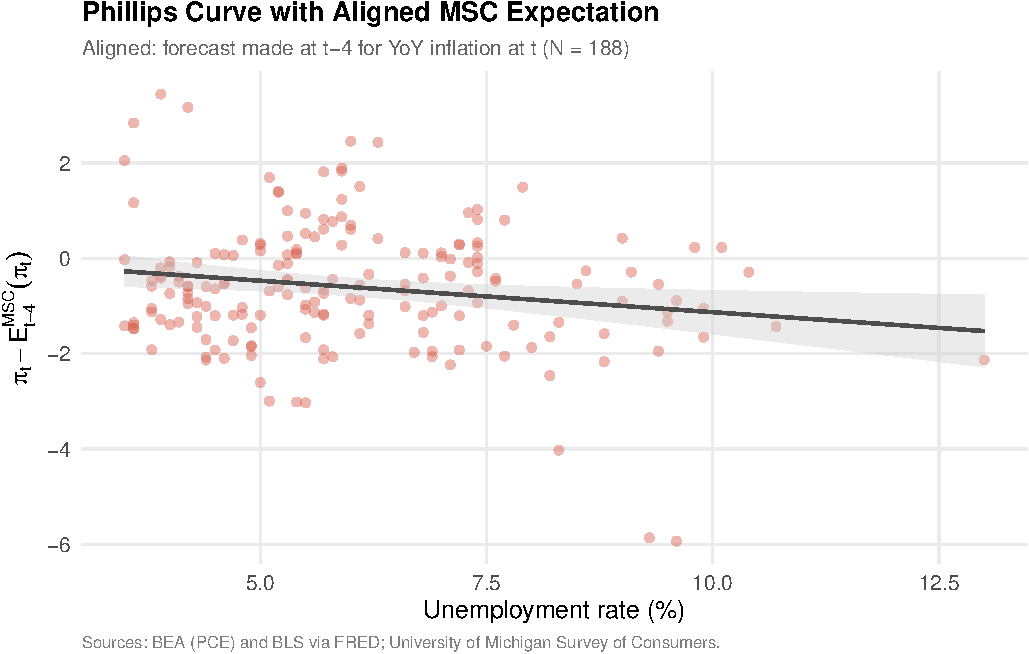
\includegraphics[width=0.9\linewidth]{../report/images/q6-msc-aligned-1} 

}

\caption{Phillips curve with the MSC forecast aligned to the realisation it predicts: $\pi_t-E^{MSC}_{t-4}[\pi_t]$.}\label{fig:q6-msc-aligned}
\end{figure}

\textbf{Answer:} When household expectations from the Michigan Survey of
Consumers are used instead of backward-looking expectations, the
Phillips curve relationship changes markedly compared to Question 2.
With the \emph{contemporaneous} specification
\(y_t = \pi_t - E^{MSC}_t[\pi_{t+4}]\) the OLS slope is small, of
indeterminate sign, and statistically indistinguishable from zero
(\(\hat{\kappa} = 0.039\) (HC1 SE \(= 0.058\)), \(R^2 = 0.004\),
\(N = 192\)); the scatterplot is essentially flat.

This result has both an economic and a measurement component. First,
household inflation expectations --- particularly since the Global
Financial Crisis --- tend to be \emph{biased upward} relative to
realised inflation, so \(\pi_t - E^{MSC}_t[\pi_{t+4}]\) is negative on
average over the sample. Second, the dependent variable as constructed
is \emph{not a properly aligned conditional surprise}: \(\pi_t\) is
current year-on-year inflation, while \(E^{MSC}_t[\pi_{t+4}]\) is a
forecast for inflation four quarters ahead. The realisation and the
forecast horizon do not match.

A simple diagnostic confirms that the timing convention matters.
Substituting \(E^{MSC}_{t-4}[\pi_t]\) --- the forecast made one year
earlier of the YoY inflation rate that has just realised --- recovers a
downward-sloping relationship (\(\hat{\kappa} = -0.132\) (HC1 SE
\(= 0.059\)), \(R^2 = 0.032\), \(N = 188\)). The slope flips from a
small positive to a small but visibly negative number once the forecast
is dated correctly, so part of the ``missing-disinflation flattening''
in the contemporaneous specification is mechanical mis-alignment rather
than evidence on the structural Phillips slope.

These findings are consistent with the central insight of Coibion and
Gorodnichenko (2015). When household expectations are used, the
phenomenon of ``missing disinflation'' essentially \emph{disappears}.
During the 2009--2013 period, household inflation expectations rose
sharply (driven by oil and gasoline prices), even as the economy was in
a deep recession. Because \(E^{MSC}_t\) was high, the inflation surprise
was already very negative --- exactly what the Phillips curve would
predict when unemployment is elevated. The ``puzzle'' arose only when
backward-looking or professional-forecaster expectations (which fell
during the recession) were used, generating a small negative surprise
inconsistent with the large unemployment gap.

\newpage

\hypertarget{question-7-simultaneity-bias-and-ols-identification}{%
\subsection{Question 7: Simultaneity Bias and OLS
Identification}\label{question-7-simultaneity-bias-and-ols-identification}}

\textbf{Answer:} A fundamental identification problem afflicts all the
OLS regressions estimated above (in Questions 2, 3, and 6):
\textbf{simultaneity (reverse causality)}. Inflation expectations and
unemployment are \emph{jointly determined} --- aggregate demand shocks
simultaneously raise inflation (or expectations thereof) and lower
unemployment, while monetary policy responses to inflation and
employment conditions shift the economy along both dimensions. OLS of
inflation on unemployment therefore conflates movements \emph{along} the
Phillips curve (driven by supply shocks, which we want to identify) with
shifts \emph{of} the Phillips curve (driven by demand shocks and policy
responses).

McLeay \& Tenreyro (2020, \emph{NBER Macroeconomics Annual} 34)
formalise this argument. They show that when the central bank conducts
\emph{optimal monetary policy} --- adjusting interest rates to stabilise
inflation in response to unemployment gaps --- the policy reaction
function induces a spurious positive correlation between inflation and
unemployment in equilibrium. This endogeneity biases the OLS estimate of
the Phillips curve slope toward zero (or even toward a positive sign).
The PC is identified \emph{only} off supply-side shocks or when an
instrumental variable for monetary policy is available.

Relating this back to our estimates:

\begin{itemize}
\tightlist
\item
  \textbf{Question 2 (Full sample, backward-looking):} The near-zero
  slope is \emph{most} susceptible to this bias. Backward-looking
  expectations move slowly and essentially proxy for lagged inflation,
  so the regression captures a mix of demand- and supply-driven
  variation, with the Fed's stabilisation policy washing out much of the
  PC signal.
\item
  \textbf{Question 3 (Subperiods):} The subperiod estimates are
  similarly biased. The observed ``flattening'' during the Great
  Moderation (1987--2007) may partly reflect a more aggressive
  inflation-targeting regime by the Fed, which offset demand shocks more
  effectively, rather than a true structural flattening of the
  underlying Phillips curve.
\item
  \textbf{Question 6 (MSC expectations):} While somewhat less biased
  because household survey expectations capture \emph{forward-looking}
  information that partially controls for demand-shock-induced
  expectation shifts, simultaneity remains. Demand booms raise both MSC
  expectations and employment, confounding the true slope estimate.
\item
  The only clean identification requires either an \emph{instrument} for
  monetary policy (e.g., narrative shocks à la Romer \& Romer) or an
  instrument for slack (e.g., Bartik-style local labour-market
  instruments, as in Gitti 2024).
\end{itemize}

\newpage

\hypertarget{section-3.3-non-linear-phillips-curves}{%
\section{Section 3.3 --- Non-linear Phillips
Curves}\label{section-3.3-non-linear-phillips-curves}}

\hypertarget{question-8-summary-of-benigno-eggertsson-2024}{%
\subsection{Question 8: Summary of Benigno \& Eggertsson
(2024)}\label{question-8-summary-of-benigno-eggertsson-2024}}

\textbf{Answer:} Benigno \& Eggertsson (2024) argue that the standard
\emph{linear} New Keynesian Phillips curve misses a critical feature of
the inflation--labour-market-tightness relationship: it is
\textbf{non-linear, exhibiting a convex (or kinked) shape}.
Specifically, they document a ``slanted-L'' pattern in the data:

\begin{itemize}
\tightlist
\item
  \textbf{At low tightness} (high unemployment, low \(V/U\)), additional
  slack has \emph{little} disinflationary effect --- the Phillips curve
  is nearly flat. This explains the ``missing disinflation'' of
  2009--2015: despite very high unemployment, inflation did not fall
  substantially because the economy was on the flat portion of the
  curve.
\item
  \textbf{At high tightness} (low unemployment, high \(V/U\)), small
  increases in tightness generate \emph{large} inflation increases ---
  the curve becomes steep, nearly vertical. This explains the rapid
  inflation surge of 2021--2022: the economy quickly moved onto the
  steep portion of the curve.
\end{itemize}

The key theoretical mechanism is a \emph{capacity constraint on
production}: firms can substitute between vacancies and labour to adjust
output, but as the labour market approaches full utilisation the
marginal cost curve becomes very steep --- effectively kinking ---
because additional output requires either bidding scarce workers away
from other firms or accepting longer vacancy durations. Once this
constraint binds, small increases in tightness map into large increases
in marginal cost and hence in price-setting markups, generating the
near-vertical arm of the slanted-L. Below the kink, by contrast,
marginal cost is roughly flat in tightness, so additional slack has
little disinflationary bite. Search-and-matching frictions are a
complementary force: when \(V/U\) is high, hiring takes longer and wage
offers must rise to attract workers, reinforcing the cost-side
amplification. Crucially, Benigno \& Eggertsson argue that \emph{no
structural break or shift in the Phillips curve is needed} to explain
both the ``missing disinflation'' and the ``inflation surge'' --- both
phenomena arise naturally from the non-linear shape of a \emph{stable}
underlying relationship.

\newpage

\hypertarget{question-9-replicating-benigno-eggertsson-2024-figure-1}{%
\subsection{Question 9: Replicating Benigno \& Eggertsson (2024) Figure
1}\label{question-9-replicating-benigno-eggertsson-2024-figure-1}}

\begin{figure}[H]

{\centering 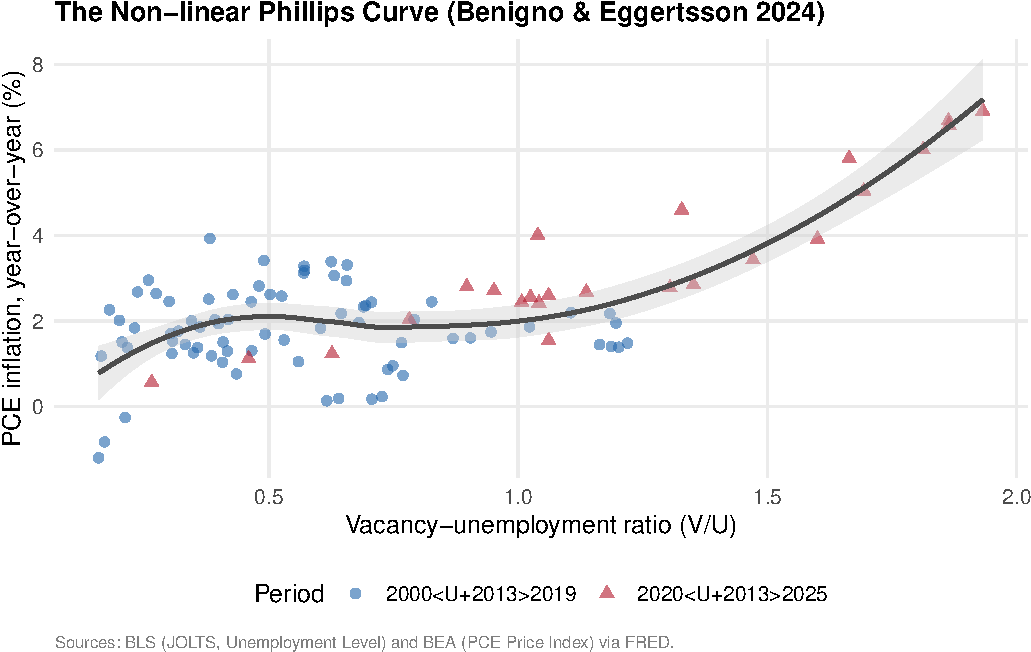
\includegraphics[width=0.9\linewidth]{../report/images/q8-nonlinear-1} 

}

\caption{Non-linear Phillips curve: PCE inflation vs.\ labour-market tightness ($V/U$).}\label{fig:q8-nonlinear}
\end{figure}

\textbf{Answer:} The scatterplot reveals the characteristic
\textbf{``slanted-L'' shape} described by Benigno \& Eggertsson (2024).
For \(V/U\) ratios below roughly \(1\), the relationship is essentially
flat: across the 2000--2019 expansion, the GFC trough, and the
late-cycle 2018--2019 quarters where \(V/U\) first crossed above one
with inflation still anchored around 2\%, year-over-year PCE inflation
hovers in a narrow \(1\)--\(2.5\%\) band regardless of tightness. The
steep, near-vertical arm of the curve is essentially the
\textbf{2021:Q2--2023:Q1 cluster}: every quarter in our sample with PCE
inflation above 4\% sits in this window, with \(V/U\) ratios between
\(1.04\) and \(1.93\). Within this cluster a roughly \(0.9\)-point
increase in \(V/U\) (from \(1.04\) to \(1.93\) over 2021:Q2--2022:Q2) is
associated with PCE inflation rising from \(4.0\%\) to \(6.9\%\). The
kink itself sits near \(V/U \approx 1\) --- close to where Benigno \&
Eggertsson place it in their Figure 1.

This pattern contrasts sharply with the \textbf{linear Phillips curve},
which would predict a uniform, moderate negative relationship between
slack and inflation across the entire range. The linear specification
would substantially overpredict disinflation during the slack post-GFC
period and underpredict inflation during the 2021--2022 boom. The
non-linear relationship shows that inflation is relatively insensitive
to tightness when the labour market has ample slack --- firms can fill
vacancies without large wage increases --- but becomes highly sensitive
once tightness pushes the economy past the kink and onto the
capacity-constrained arm. As the post-2022 observations show, the
unwinding of tightness brought inflation back down, tracing the curve in
reverse: the 2024--2025 quarters are back at \(V/U\approx 1\) with PCE
inflation around \(2.5\%\).

\newpage

\hypertarget{question-10-summary-of-gitti-2024}{%
\subsection{Question 10: Summary of Gitti
(2024)}\label{question-10-summary-of-gitti-2024}}

\textbf{Answer:} Gitti (2024) addresses a key \textbf{endogeneity
concern} that plagues the OLS scatterplot in Question 9: the
vacancy-unemployment ratio \(V/U\) is endogenous to inflation because
demand shocks simultaneously raise both labour-market tightness and
prices. Her identification strategy uses a \textbf{Bartik-style
(shift-share) instrumental variable}: she exploits the fact that local
labour markets are differentially exposed to national industry-level
vacancy shocks. By interacting pre-determined local industry employment
shares (the ``shares'') with national industry-level vacancy changes
(the ``shifts''), she constructs an instrument that captures exogenous
variation in local tightness that is plausibly uncorrelated with local
demand shocks.

This approach relates directly to Question 9 (and Question 7): the OLS
scatterplot is subject to the \textbf{same simultaneity bias} discussed
previously. During demand booms, both tightness and inflation rise
\emph{simultaneously}, inflating the apparent slope of the
tightness--inflation relationship. Conversely, during recessions, both
decline together. The OLS estimates therefore confound the causal effect
of tightness on inflation with the common response of both variables to
demand conditions.

Gitti's IV strategy recovers a \textbf{cleaner causal estimate} of the
tightness--inflation relationship, which she finds to be:

\begin{enumerate}
\def\labelenumi{\arabic{enumi}.}
\tightlist
\item
  \textbf{Non-linear}, consistent with the slanted-L shape documented by
  Benigno \& Eggertsson (2024);
\item
  \textbf{Quantitatively different} from OLS --- the IV estimates
  suggest the true causal relationship is steeper in the tight-market
  region than OLS implies (because OLS averages over demand- and
  supply-driven variation);
\item
  \textbf{Robust} to controlling for local demand conditions and to
  various specification checks on the instrument's validity.
\end{enumerate}

Her results thus provide rigorous causal support for the non-linear
Phillips curve hypothesis and demonstrate that naive OLS estimates ---
whether using unemployment (Q2, Q5) or tightness (Q8) --- are biased by
simultaneity.

\newpage

\hypertarget{appendix}{%
\section{Appendix}\label{appendix}}

\begin{verbatim}
R version 4.4.2 (2024-10-31)
Platform: aarch64-apple-darwin20
Running under: macOS 26.3.1

Matrix products: default
BLAS:   /Library/Frameworks/R.framework/Versions/4.4-arm64/Resources/lib/libRblas.0.dylib 
LAPACK: /Library/Frameworks/R.framework/Versions/4.4-arm64/Resources/lib/libRlapack.dylib;  LAPACK version 3.12.0

locale:
[1] C

time zone: Europe/Rome
tzcode source: internal

attached base packages:
[1] stats     graphics  grDevices utils     datasets  methods   base     

other attached packages:
 [1] lmtest_0.9-40      zoo_1.8-15         sandwich_3.1-1     dotenv_1.0.3      
 [5] kableExtra_1.4.0   scales_1.4.0       modelsummary_2.5.0 fredr_2.1.0       
 [9] lubridate_1.9.4    forcats_1.0.0      stringr_1.5.1      dplyr_1.2.0       
[13] purrr_1.0.4        readr_2.1.5        tidyr_1.3.1        tibble_3.3.1      
[17] ggplot2_4.0.2      tidyverse_2.0.0   

loaded via a namespace (and not attached):
 [1] gtable_0.3.6       xfun_0.52          lattice_0.22-6     tzdb_0.5.0        
 [5] vctrs_0.7.2        tools_4.4.2        generics_0.1.4     curl_6.2.2        
 [9] parallel_4.4.2     pkgconfig_2.0.3    Matrix_1.7-3       data.table_1.18.0 
[13] RColorBrewer_1.1-3 S7_0.2.1           lifecycle_1.0.5    compiler_4.4.2    
[17] farver_2.1.2       textshaping_1.0.0  tinytex_0.54       htmltools_0.5.8.1 
[21] yaml_2.3.10        pillar_1.11.1      crayon_1.5.3       nlme_3.1-167      
[25] tidyselect_1.2.1   digest_0.6.37      stringi_1.8.4      labeling_0.4.3    
[29] splines_4.4.2      rprojroot_2.1.1    fastmap_1.2.0      grid_4.4.2        
[33] here_1.0.2         cli_3.6.5          magrittr_2.0.4     withr_3.0.2       
[37] bit64_4.6.0-1      timechange_0.3.0   rmarkdown_2.29     httr_1.4.7        
[41] bit_4.5.0.1        hms_1.1.3          evaluate_1.0.3     knitr_1.49        
[45] viridisLite_0.4.3  mgcv_1.9-1         rlang_1.1.7        glue_1.8.0        
[49] xml2_1.3.6         svglite_2.2.2      rstudioapi_0.17.1  vroom_1.6.5       
[53] jsonlite_1.8.9     R6_2.6.1           tables_0.9.33      systemfonts_1.3.1 
\end{verbatim}

\end{document}
